\begin{frame}[c] \frametitle{ Zero-based guards }
	\vspace{-5pt}
	\begin{block}{Definition}
		A zero-based guard is a constraint expressed in a specific format in Equation~\eqref{eq:zero-based-form}.
		\begin{equation}
			g(X(t), I(t)) \otimes 0, \quad \otimes \in \{<, >, \leq, \geq, == \}
			\label{eq:zero-based-form}
		\end{equation}
		$g(X(t), I(t))$ is called a \emph{guard trace}. Consider it as a signal evolving over time. By abuse of notation, we denote $g(t)$. Naturally, solving it for $t$ gives the values satisfying the guard. 
	\end{block}
	
	\begin{block}{Proposition}
		Any guard can be easily expressed in the zero-based format.\\
		\emph{Proof.} Rearrange the constraint to move everything to the left-hand side.
	\end{block}
	 
	\begin{block}{Example}
		A nonlinear guard: $ 3x + 4xy > (x+1)^2$ \\
		Zero-based form: $ 3x + 4xy - (x+1)^2 > 0$
	\end{block}
\end{frame}

\begin{frame}[c] \frametitle{ Guard-Dependent Dynamic Quantum }
	\begin{block}{Definition: Quantum }
		In QSS, simulation step is invoked based on a signal $x(t)$ and a quantum $\Delta q_x$.
		\begin{equation}
			| x(t) - x(t_0) | = \Delta q_x, \quad \therefore x(t) = x(t_0) \pm \Delta q_x
		\end{equation}
	\end{block}
	
	\begin{block}{ Dynamic Quantum }
		Similar to QSS, we have $g(t) = g(t_0) \pm \Delta q_g$ \\
		We set the quantum based on the guard $\Delta q_g = g(t_0)$\\
		Now, we need to solve:
		\begin{itemize}
			\item $g(t) = 0$, equivalent to solving the guard constraint.
			\item $g(t) = 2 g(t_0)$, when the guard trace moves away from the zero line.
		\end{itemize}	
	\end{block}
\end{frame}

\begin{frame}[c] \frametitle{ Guard-Dependent Dynamic Quantum (Cont.) }
	\begin{figure}
		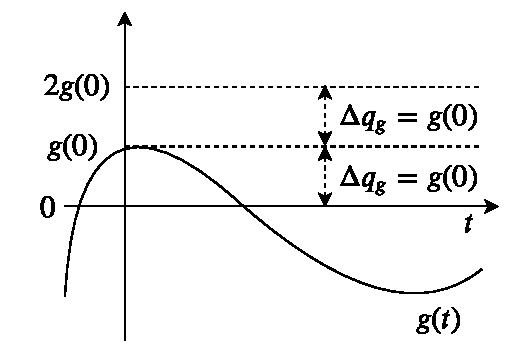
\includegraphics[width=0.7\textwidth]{./fig/diagrams/deltaq.pdf}
	\end{figure}
\end{frame}

\begin{frame}[c] \frametitle{ Taylor expansion of zero-based guards }
	\begin{block}{Description}
		To avoid expensive computation, we want to solve $g(t)$ in polynomial complexity. By abuse of notation, we denote:
		\begin{itemize}
			\item 1st-derivative: $g^{(1)}(t) = \dfrac{d}{dt} \big( g(X(t), I(t)) \big)$
			\item 2nd-derivative: $g^{(2)}(t) = \dfrac{d^2}{dt^2} \big( g(X(t), I(t)) \big)$
		\end{itemize}
		Then, the Taylor polynomials of the guard at time $t_0$ is:
		\begin{equation}
			g(t) = g(t_0) + \mathlarger{\sum}_{n=1}^{\infty} \dfrac{g^{(n)}(t_0)}{n!} \cdot (t - t_0)^n
		\end{equation}
	\end{block}
\end{frame}

\begin{frame}[c] \frametitle{ Theorem: solving a guard always has at least one real root }
	\begin{block}{Lemma}
		Let $0 = a_n x^n + a_{n-1} x^{n-1} + ... + ax \pm c$, be a polynomial of degree $n$ with real coefficients. Then, $f(x)$ has at least one real positive root.
	\end{block}
	\begin{block}{proof}
		Let $m \in \mathbb{Z}^{\geq 0}$ be the number of sign changes within the sequence $(a_n,...,a)$ (i.e., without considering $\pm c$). The possible values of $m \in [0,n-1]$. Descartes' rule of signs states that, if there are $m$ number of sign changes, then there are exactly $m$ real positive roots or less but an odd number of roots. 
		\begin{itemize}
			\item Case $m \geq 1$: regardless of considering the sign of $\pm c$, there is always at least one real positive root by Descartes' rule of signs. 
			\item Case $m = 0$: since $\pm c$ can be either signs, there is always a sign change between $a$ and $c$. Thus, there is at least one real positive root.
		\end{itemize}
	\end{block}
\end{frame}

\begin{frame}[c] \frametitle{ Theorem: solving a guard always has at least one real root (Cont.) }
	\begin{block}{Theorem}
		Let $g(t)$ be a Taylor polynomials of $n$ degree. Then, solving either $g(t) = 0$ or $g(t) = 2g(t_0)$ always result in at least one real positive root.
	\end{block}
	\begin{block}{proof}
		\begin{itemize}
			\item Case $g(t) = 0$: we have $0 = g(t_0) + \mathlarger{\sum}_{n=1}^{\infty} \dfrac{g^{(n)}(t_0)}{n!} \cdot (t - t_0)^n$. 
			\item Case $g(t) = 2g(t_0)$: we have $0 = -g(t_0) + \mathlarger{\sum}_{n=1}^{\infty} \dfrac{g^{(n)}(t_0)}{n!} \cdot (t - t_0)^n$.
		\end{itemize}
		Combining two cases, we have $0 = \pm g(t_0) + \mathlarger{\sum}_{n=1}^{\infty} \dfrac{g^{(n)}(t_0)}{n!} \cdot (t - t_0)^n$. Therefore, the previous Lemma applies directly.
	\end{block}
\end{frame}

\begin{frame}[c] \frametitle{ Finding the first positive real root }
	\begin{algorithm}[H]
	\SetAlgoLined
	\SetKwInOut{Function}{Function}
	\SetKwInOut{Input}{Input}
	\SetKwInOut{Output}{Output}
	\Function{FirstRoot}
	\Input{$\vec{X}$ cont vars smooth tokens, $\vec{I}$ input var smooth tokens, and the guard $g$.}
	\Output{the first root $t_{f}$}
	TaylorCoeff $\leftarrow$ ComputeDerivatives($g(t)$, $\vec{X}$, $\vec{I}$)\;
	Roots $\leftarrow$ Solve(TaylorCoeff)\;
	\ForEach{$r \in $Roots $\wedge$ $r < 0$}{
		Roots.pop($r$)\;	
	}
	$t_f \leftarrow $ min(Roots)\;
	\caption{Computing the first positive real root}
	\end{algorithm}
\end{frame}


\begin{frame}[c] \frametitle{ Approximation validity checking using local truncation error }
	\begin{block}{Local Truncation Error Definition}
		For a signal $x(t)$, let $x^h(t)$ be a precise approximation (i.e., $n$th order), and $x^l(t)$ be a relatively less precise approximation (i.e., $n-1$th order). Then. local truncation error $LTE_x(t)$ is:
		\begin{equation}
			LTE_x(t) = | x^h(t) - x^l(t) |
		\end{equation}
	\end{block}
	\begin{block}{Lemma}
		Local truncation error of the guard $g(t)$ is equivalent to the last term (i.e., highest order) polynomial term. 
		\begin{equation}
			LTE_g(t) = \dfrac{| g^{(n)}(t_0) |}{n!}(t-t_0)^n
		\end{equation}
		If we want to ensure a certain LTE,
		\begin{equation}
			t = \sqrt[n]{\dfrac{LTE \times n!}{ |g^{(n)}(t_0)|}} + t_0
		\end{equation}
	\end{block}
\end{frame}

\begin{frame}[c] \frametitle{ Approximation validity checking using local truncation error (cont.) }
	\begin{block}{proof}
		Consider $n$th order $g(t)$. We have a high and low order approximations: 
		\begin{gather}
			g^h(t) = g(t_0) + \mathlarger{\sum}_{i=1}^{n} \dfrac{g^{(i)}(t_0)}{i!} \cdot (t - t_0)^i \\
			g^l(t) = g(t_0) + \mathlarger{\sum}_{i=1}^{n-1} \dfrac{g^{(i)}(t_0)}{i!} \cdot (t - t_0)^i 	\\			
		\end{gather}
		Therefore, we have:
		\begin{equation}
			LTE_g(t) = | g^h(t) - g^l(t) | = \dfrac{ | g^{(n)}(t_0)|}{n!}(t-t_0)^n		
		\end{equation}
	\end{block}
\end{frame}

\begin{frame}[c] \frametitle{ Computing the step size $\delta$ }
	\begin{algorithm}[H]
	\SetAlgoLined
	\SetKwInOut{Input}{Input}
	\SetKwInOut{Output}{Output}
	\Input{$\vec{X}$, $\vec{I}$, and list of guards $G$}
	\Output{Step size $\delta$}
	$\xi \leftarrow \phi$\;
	\ForEach{ var $\in \vec{X} \cup \vec{I}$}{
		$t_{var} \leftarrow$ ValidTime(var, $k$)\;
		$\xi$.append($t_{var}$)\;
	}
	\ForEach{guard $g$ from the current location}{
		$t_r \leftarrow$ firstRoot($g, \vec{X}, \vec{I}$)\;
		$t_{val}\leftarrow $ ValidTime($g$, $k$)\;
		$t_{grd} \leftarrow$ min($t_r, t_{val}$)\;
		$\xi$.append($t_{grd}$)\;
	}
	$\delta \leftarrow $ min($\xi$)\;
	\caption{ $\delta$ computation }
	\end{algorithm}
\end{frame}

\begin{frame}[c] \frametitle{ Bounded local truncation error }
	\begin{block}{Lemma}
		The local truncation error value is monotonically increasing over time such that for any two time values $t_1$ and $t_2$ such that $t_1 < t_2$, then $LTE(t_1) < LTE(t_2)$ is always true.
	\end{block}
	\begin{block}{proof}
		We can directly prove this by considering $LTE_g(t_2) - LTE_g(t_1) > 0$. \\ 
		Since $LTE_g(t) = \dfrac{|g^{(n)}(t_0)|}{n!}(t-t_0)^n$, \\ 
		$LTE_g(t_2) - LTE_g(t_1) > 0 \implies \dfrac{|g^{(n)}(t_0)|}{n!} \bigg( (t_2-t_0)^n - (t_1-t_0)^n \bigg) > 0 $ \\
		$\because \dfrac{|g^{(n)}(t_0)|}{n!} > 0, \quad (t_2-t_0)^n - (t_1-t_0)^n > 0$ needs to be true. \\
		$t_2 > t_1 > t_0 > 0, \quad \therefore (t_2- t_0) > 0 \wedge (t_1 - t_0) > 0 \wedge (t_2- t_0) > (t_1- t_0)$. \\
		Consequently, $(t_2-t_0)^n - (t_1-t_0)^n > 0$ is always true. \\
		Therefore, $LTE_g(t_2) - LTE_g(t_1) > 0$ is always true.
	\end{block}
	
\end{frame}

\begin{frame}[c] \frametitle{ Bounded local truncation error (cont.) }
	\begin{block}{Theorem}
		The computed $\delta$ at time $t_0$ in Algorithm 2 guarantees, for any state variable $x$, the local truncation error $LTE_x(t)$ is bounded such that $LTE_x(t) \leq k$ is satisfied for $\forall t \in [t_0, t_0 + \delta]$, where $k$ is the user specified constant.
	\end{block}
	\begin{block}{proof}
		Without loss of generality, we assume $t_0 = 0$. For any arbitrarily chosen variable $x$, we have $t_x =$ ValidTime($x$, $k$) in Algorithm 2. Since $\delta$ is assigned to the minimum value, $\delta$ can be either equal to or less than $t_x$.
		\begin{itemize}
			\item Case $t_x = \delta$: $LTE_x(t_x) = k = LTE_x(\delta)$. $\forall t \in [0, \delta]$, by the previous Lemma, $LTE_x(t) \leq LTE_x(\delta)$. Hence, $LTE_x(t) \leq k$.
			\item Case $t_x > \delta$: by the previous Lemma, $LTE_x(\delta) < LTE_x(t_x) = k$ holds. Furthermore, $\forall t \in [0, \delta]$, $LTE_x(t) \leq LTE_x(\delta) < LTE_x(t_x) = k$.
		\end{itemize}
	\end{block}
\end{frame}

\begin{frame}[c] \frametitle{ Simulation Execution Algorithm }
	\begin{algorithm}[H]
	\SetAlgoLined
	\SetKwInOut{Input}{Input}
	\SetKwInOut{Output}{Output}
	\Input{List of HIOA/PDs $Q$, List of connectors $C$}
	\Output{The output traces $Trac$}
	 initialization($Q$)\;
	 $time \leftarrow 0$\;
	 \While{$time \leq T_{max}$}{
	  InterLocation($Q$)\;
	  $Trac$.append($time$, getOutputValues($Q$)\;
	  
	  \lForEach{connector $c \in C$}{ExchangeTokens($c, Q$)}
	  \lForEach{$HIOA^+$ object $q \in Q$}{	  $\delta$.append(ComputeDelta($q$))}

	  $\delta_{step} \leftarrow $ min($\delta$)\;
	  \eIf{ $time + \delta_{step} > T_{max}$ }{
		$time \leftarrow T_{max}$
	  }{
		$time \leftarrow$ time $+ \delta_{step}$
	  }
	  
	 }
	 \caption{Simulation Execution Pseudo Code}
	\end{algorithm}
\end{frame}
